\documentclass[a4paper,12pt]{article} % declaration
\usepackage[utf8]{inputenc}
\usepackage{amsmath}
\usepackage{amsthm,accents}
\usepackage{amsfonts}
\usepackage{color}
\usepackage{graphicx}
\usepackage{tikz}
\usepackage{lmodern,bm}
\usepackage{enumitem}

\newtheorem{definition}{Definition}[section]
\newtheorem{theorem}{Theorem}[section]
\newtheorem{proposition}{Proposition}[section]
\newtheorem{lemma}[theorem]{Lemma}
\newtheorem{corollary}[theorem]{Corollary}
\newtheorem{example}{Examples}
\newtheorem*{remark}{Remark}
\title{Mean Value Theorem}
\author{Guoning Wu}
\begin{document}
\tableofcontents
\setcounter{tocdepth}{2}
\listoffigures
\listoftables
\maketitle

\theoremstyle{definition}

\section{Fermat's Lemma and Rolle's Theorem}
\begin{definition}
    \normalfont A point $x_0 \in E \subset \mathbb{R}$ is called a local maximum (resp. local minimum) and 
    the value of a function of a function $f: E \to \mathbb{R}$ at that point a local 
    maximum value (resp. local minimum value) if there exists a neighborhood $U_E(x_0)$
    in $E$ such that at any point $x \in U_E(x_0)$ we have $f(x) \le f(x_0)$ (resp. $f(x) \ge f(x_0)$.
\end{definition}

\begin{definition}
    \normalfont If the strict inequality $f(x) < f(x_0)$(resp. $f(x) > f(x_0)$) holds at every point 
    $x \in U_E(x_0)\setminus x_0$, the point $x_0$ is called strict local maximum (resp. strict local
    minimum) and the value of the function $f: E \to \mathbb{R}$ a strict local maximum 
    value (resp. strict local minimum value).
\end{definition}

\begin{definition}
    \normalfont The local maxima and minima are called local extrema and the values of the function
    as these extreme values of the function.
\end{definition}

\begin{example}
    \[
        f(x) = \left\{\begin{array}{rcl} x^2 & \mbox{for} & -1 \le x < 2\\
                                   4  & \mbox{for} & 2 \le x
                \end{array} \right.
                \]
\end{example}

\begin{example}
    Let $f(x) = \sin \frac{1}{x}$ on set $E = \mathbb{R}\setminus 0.$
\end{example}

\begin{lemma}{\mbox{(Fermat)}}
    \normalfont If a function $f: E \to \mathbb{R}$ is differentiable at an interior 
    extremum, $x_0 \in E$, then its derivative at $x_0$ is $0: f'(x_0) = 0$.
\end{lemma}

\begin{remark}
    \normalfont 
    \begin{enumerate}
        \item Fermat's theorem thus gives a necessary condition for an interior
            extremum of differentiable function. For non-interior extrema it is 
            generally not true that $f'(x_0) \ne 0$.
        \item Geometrically this lemma is obvious, since it asserts that an extremum 
            of a differentiable function the tangent to its graph is horizontal.
        \item Physically this lemma means that in motion along a line the velocity 
            must be zero at the instant when the direction reverses.
    \end{enumerate}
\end{remark}

\begin{proposition}{\rm \textbf{(Rolle's Theorem)}}
    \rm If a function $f: [a,b] \to \mathbb{R}$ is continuous on a closed 
    interval $[a,b]$ and differentiable on the open set $]a,b[$ and $f(a) = f(b)$,
    then there exists a point $\xi \in ]a,b[$ such that $f'(\xi) = 0$.
\end{proposition}

\section{The theorems of Lagrange and Cauchy on finite increments}
The following proposition is one of the most frequently used and important methods 
of studying numerical-valued functions.

\begin{theorem}{\rm \textbf{(Lagrange's finite-increment theorem)}}
    \normalfont If a function $f: [a,b] \to \mathbb{R}$ is continuous on a closed 
    interval $[a,b]$ and differentiable on the open interval $]a,b[$, there 
    exists a point $\xi \in ]a,b[$ such that 
    \begin{equation}
        f(b) - f(a) = f'(\xi)(b-a)
        \label{eq:eq1}
    \end{equation}
\end{theorem}

\graphicspath{
    {./Figs/}
}
\begin{figure}[htbp]
    \centering
    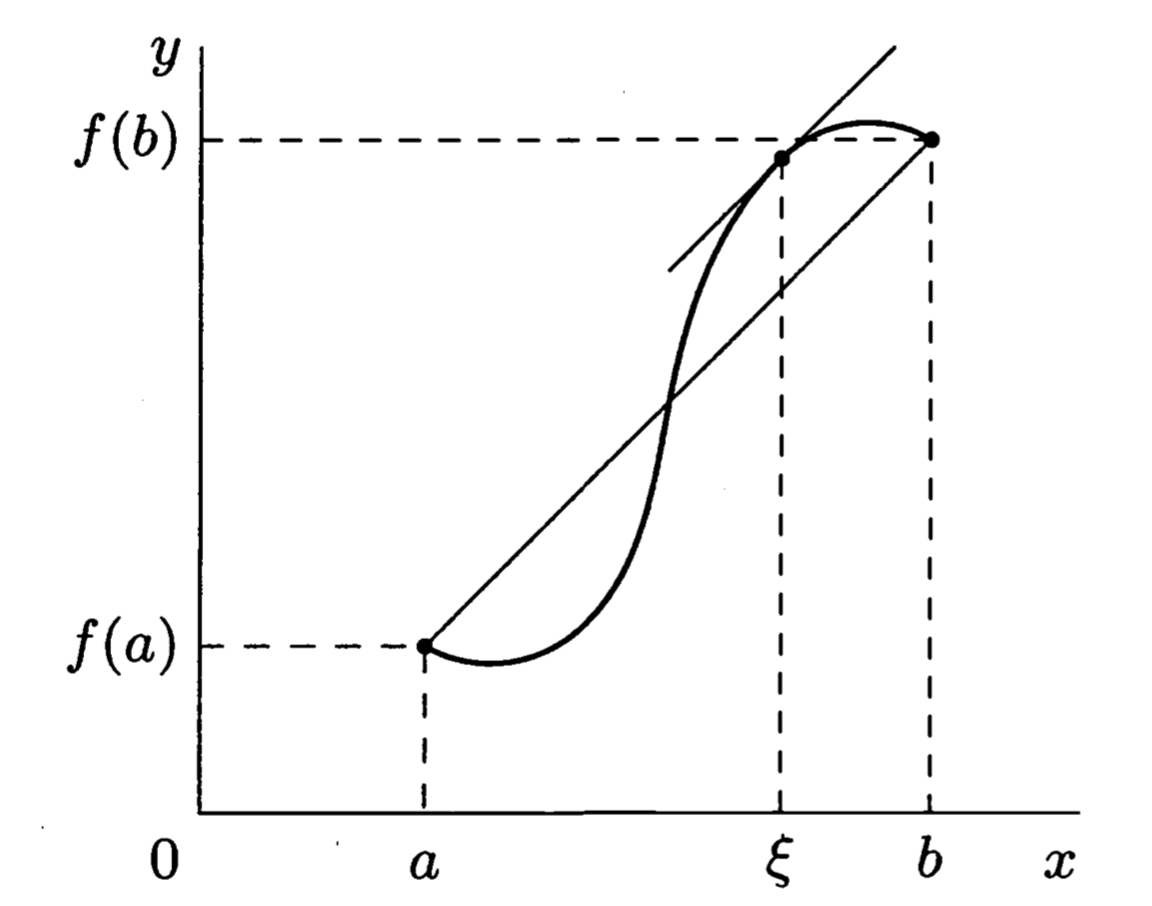
\includegraphics[width=0.5\textwidth,height=0.4\textwidth]{lagrange.png}
    \caption{Lagrange's finite-increment theorem}
    \label{fig:lagrange}
\end{figure}

\begin{remark}
    \normalfont
    \begin{enumerate}
        \item In geometric language Lagrange's theorem means that at some 
            point $(\xi, f(\xi))$, where $\xi \in ]a,b[$ the tangent to the 
            graph of the function is parallel to the chord joining the 
            points $(a,f(a))$ and $(b,f(b))$, since the slope of the chord equals 
            $\frac{f(b) - f(a)}{b - a}$.
        \item If $x$ is interpreted as time and $f(b) - f(a)$ as the amount of 
            displacement over the time $b - a$ of a particle moving along a line,
            Lagrange's theorem says that the velocity at some time $\xi \in ]a,b[$
            is the average velocity.
        \item We note nevertheless that for motion that is not along a straight 
            line there may be no average in the sense of Remark. Indeed, suppose 
            the particle is moving a circle of unit radius at constant angular 
            velocity $\omega = 1$. Its law of motion, as we know, can be written as 
            \[
                \bm{r}(t) = \left(\cos t, \sin t\right). 
                \]
            Then 
            \[
                \dot{\bm{a}}(t) = (\cos t, \sin t)
                \]
            and 
            \[
                \vert \bm{v} \vert = 1
                \]
    \end{enumerate}
\end{remark}

The particle is at the same pint $\bm{r}(0) = \bm{r}(2\pi)$, the equality 
means that 
\[
    \bm{r}(2\pi)  - \bm{r}(0) = \bm{v}(\xi)(2\pi - 0)
    \]
would mean $t=2\pi $. But this is impossible.

Even so, we shall learn that there is still a relation between the 
displacement over a time interval and velocity. It consists of the 
fact that the full length of the path traversed cannot exceed the 
maximal absolute vale of the velocity multiplied by the time interval 
of the displacement.
\begin{equation}
    \vert \bm{r}(b) - \bm{r}(a) \vert \le \sup_{t \in [a,b]} \vert 
    \dot{\bm{r}}(t)\vert \vert b-a\vert. 
\end{equation}

As will be shown later, this natural inequality does indeed always 
hold. It is also called \textbf{Lagrange's finite-increment theorem},
while relation\ref{eq:eq1} is often called \textbf{Lagrange mean value
theorem}(the role of the mean in this case is played by both the 
value $f'(\xi)$ of the velocity and by the point $\xi$ between $a$  and $b$).

\begin{corollary}
    \normalfont If the derivative of a function in non-negative (resp. 
    positive) at every point of an open interval, then the function is 
    non-decreasing (resp. increasing) on that interval.
\end{corollary}

\begin{corollary}
    \normalfont
    A function that is continuous on a closed interval $[a,b]$ is constant 
    on it if and only if its derivative equals zero at every point of the 
    interval $[a,b]$(or only the open interval $(a,b)$).
\end{corollary}

\begin{proposition}{\rm (Cauchy's finite-increment theorem)}
    \normalfont Let $x = x(t)$ and $y = y(t)$ be functions that are continuous 
    on a closed interval $[a,b]$ and differentiable on the open interval $]a,b[$.
    Then there exists a point $\tau \in [a,b]$ such that 
    \[
        x'(\tau)(y(b) - y(a)) = y'(\tau)(x(b) - x(a))
        \]
    If in addition $x'(t) \ne 0$ for each $t \in ]a,b[$, then $x(a) \ne x(b)$
    and we have the equality 
    \[
        \frac{y(b) - y(a)}{x(b) - x(a)} = \frac{y'(\tau)}{x'(\tau)}
        \]
\end{proposition}

\section{Taylor's Formula}
If we are given a function $f(x)$ having derivatives up to order $n$
inclusive at $x_0$, we can immediately write the polynomial
\begin{equation}
    P_n(x_0;x) = P_n(x) = f(x_0) + \frac{f'(x_0)}{1!}(x - x_0) + 
    \cdots + \frac{f^{(n)}(x_0)}{n!}(x - x_0)^n,
    \label{eq:eq2}
\end{equation}
whose derivatives up to order $n$ at the point $x_0$ are the same as 
as the corresponding derivatives of $f(x)$ at that point.

\begin{definition}
    \normalfont The algebraic polynomial given by Eq.~\ref{eq:eq2} is the 
    Taylor polynomial of order $n$ of $f(x)$ at $x_0$.
\end{definition}

We shall be interested in the value of 
\begin{equation}
    f(x) - P_n(x_0;x) = r_n(x_0;x),
\end{equation}
of the discrepancy between the polynomial $P_n(x)$ and the function $f(x)$,
which is often called the remainder, more precisely, the $n$th remainder 
or the $n$th remainder term in Taylor's formula:
\[
    f(x) = f(x_0) + \frac{f'(x_0)}{1!}(x - x_0) + 
    \cdots + \frac{f^{(n)}(x_0)}{n!}(x - x_0)^n + r_n(x_0;x)
    \]
\begin{theorem}
    \normalfont
    If the function $f$ is continuous on the closed interval with end
    points $x_0$ and $x$ along with its first $n$ derivatives, and it has a 
    derivative of order $n+1$ at the interior points of this interval, 
    then for any function $\phi$ that is continuous on this closed interval 
    and has a nonzero derivative at its interior points, there exists 
    a point $\xi$ between $x_0$ and $x$ such that 
    \begin{equation}
        r_n(x_0;x) = \frac{\phi(x) - \phi(x_0)}{\phi'(\xi)n!}f^{(n+1)}(\xi)(x-\xi)^n
    \end{equation}
\end{theorem}

\textbf{Proof:}  On the closed interval $I$  with endpoints $x_0$ and $x$ we consider 
the auxiliary function
\[
    \begin{split}
        F(t) &= f(x) - P(t;x)\\
        & \frac{F(x) - F(x_0)}{\phi(x) - \phi(x_0)} = \frac{F'(\xi)}{\phi'(\xi)}
    \end{split}
    \]
Setting $\phi(t) = x-t$, we obtain the following corollary,
\begin{corollary}{\rm (Cauchy's formula for the remainder term)}
    \[
        r_n(x_0;x) = \frac{1}{n!}f^{(n+1)}(\xi)(x-\xi)^{n+1}(x - x_0)
        \]
\end{corollary}

A particular elegant formula results if we set $\phi(t) = (x-t)^{n+1}$.
\begin{corollary}{\rm (Lagrange's form for the remainder term)}
    \[
        r_n(x_0; x) = \frac{1}{(n+1)!}f^{(n+1)}(\xi)(x - x_0)^{n+1}.
        \]
\end{corollary}

Let us consider some examples.
\begin{example}
    \normalfont
    For the function $f(x) = e^x$ with $x_0 = 0$ Taylor's formula has
    the form
    \[
        e^x = 1 + \frac{1}{1!}x^2 + \frac{1}{2!}x^2 + \cdots + \frac{1}{n!}x^n + r_n(0;x)
        \]
    and the remainder is 
    \[
        r_n(0;x) = \frac{1}{(n+1)!}e^{\xi}x^{n+1}
        \]
    where $\vert \xi \vert < \vert x \vert$  .
    Thus 
    \[
        \vert r_n(0;x)\vert  = \frac{1}{(n+1)!}e^{\xi}\vert x \vert^{n+1} < \frac{\vert x \vert^{n+1}}{(n+1)!}e^{\vert x \vert}.
        \]
    But for each fixed $x \in \mathbb{R}$, if $n \to \infty$, the quantity $\frac{\vert x \vert^{n+1}}{(n+1)!}$ , as we know ,
    tends to zero. Hence 
    \[
        e^x = 1 + \frac{1}{1!}x + \frac{1}{2!}x^2 + \cdots + \frac{1}{n!}x^n + \cdots, \forall x \in \mathbb{R}
\]
\end{example}

\begin{example}
    \normalfont
    The function $a^x, 0<a, a\ne 1$, similarly:
    \[
        a^x = 1 + \frac{\ln a}{1!}x + \frac{\ln^2a}{2!}x^2 + \cdots + \frac{\ln^na}{n!}x^n + \cdots
        \]
\end{example}

\begin{example}
    \[
        \sin x = x - \frac{1}{3!}x^3 + \frac{1}{5!}x^5 + \cdots + \frac{(-1)^n}{(2n+1)!}x^{2n+1} + \cdots
        \]
\end{example}

\begin{example}
    \[
        \cos x = 1 - \frac{1}{2!}x^2 + \frac{1}{4!}x^4 + \cdots + \frac{(-1)^n}{(2n)!}x^{2n} + \cdots, \forall x \in \mathbb{R}
        \]
\end{example}

\begin{example}
    \[
        \sinh x = x + \frac{1}{3!}x^3 + \frac{1}{5!}x^5 + \cdots + \frac{1}{(2n+1)!}x^{2n+1}+ \cdots, \forall x \in \mathbb{R}
        \]
\end{example}
\begin{example}
    \[
        \cosh x = 1 + \frac{1}{2!}x^2 + \frac{1}{4!}x^4 + \cdots + \frac{1}{(2n)!}x^{2n}+ \cdots, \forall x \in \mathbb{R}
        \]
\end{example}

\begin{example}
    \normalfont
    For the function $f(x) = \ln (1+x)$, we have 
    \[
        \ln (1+x) = x - \frac{1}{2}x^2 + \frac{1}{3}x^3 + \cdots + \frac{(-1)^{(n-1)}}{n}x^n + r_n(0;x).
        \]
    where 
    \[
        r_n(0;x) = \frac{1}{n!}\frac{(-1)^nn!}{(1+\xi)^{n+1}}(x - \xi)^nx,
        \]
    or 
    \[
        r_n(0;x) = (-1)^nx\frac{(x - \xi)^n}{(1+\xi)^n}\frac{1}{(1+\xi)}
        \]
    where $\xi$ lies between $0$ and $x$.

    If $\vert x \vert < 1$, it follows from the condition that $\xi $  lies between $0$ and $x$ that 
    \[
        \frac{\vert x - \xi \vert}{\vert 1 + \xi \vert}  = \frac{\vert x \vert - \vert \xi \vert}{1 - \vert \xi \vert} 
        = 1 - \frac{1 - \vert x \vert}{1 - \vert \xi \vert} \le 1 - \frac{1 - \vert x \vert}{1 - \vert 0 \vert} 
        = \vert x \vert.
        \]
    Thus for $\vert x \vert$ < 1
    \[
        \vert r_n(0;x) \vert \le \vert x \vert^{n+1},
        \]
    and consequently the following expansion is valid for $\vert x \vert < 1$:
    \[
        \ln (1+x) = x - \frac{1}{2}x^2 + \frac{1}{3}x^3 + \cdots + \frac{(-1)^n}{n}x^n + \cdots
        \]
\end{example}

\begin{example}
    \normalfont
    For the function $(1+x)^{\alpha}$, where $\alpha \in \mathbb{R}$, we have 
    $\displaystyle f^{(n)}(x) = \alpha(\alpha - 1)(\alpha - 2)\cdots(\alpha - n + 1)(1+x)^{\alpha - n} $,
    so that the Talylor's formula at $x_0 = 0$ for this function has the 
    form 
    \begin{equation}
        (1+x)^{\alpha} = 1 + \frac{\alpha}{1!}x + \frac{\alpha(\alpha - 1)}{2!} 
        + \cdots + \frac{\alpha(\alpha-1)\cdots(\alpha-n+1)}{n!}x^n + r_n(0;x)
    \end{equation}
    Using Cauchy's remainder, we find 
    \[
        r_n(0;x) = \frac{\alpha(\alpha-1)\cdots(\alpha-n)}{n!}(1+\xi)^{\alpha - n -1}
        (x - \xi)^nx,
        \]
    where $\xi$ lies between $x$.

    If $\vert x \vert < 1$,then, using the estimates, we have
    \begin{equation}
        \vert r_n(0;x) \vert \le \left\vert \alpha \left(1-\frac{\alpha}{1}\right)
        \cdots \left(1-\frac{\alpha}{n}\right)\right\vert \left(1+\xi\right)^{\alpha-1} 
        \vert x \vert^{n+1}.
        \label{eq:eq3}
    \end{equation}
    When $n$ is increased by 1, the right side of Eq.~\ref{eq:eq3}
    is multiplied by $\displaystyle \left\vert \left(1 - \frac{\alpha}{n+1}\right)
    x\right\vert$. But since $\vert x \vert < 1$, we shall have 
    $\left\vert\left(1 - \frac{\alpha}{n+1}\right)x\right\vert < q < 1$,
    independently of the value $\alpha$, provided $\vert x \vert < q < 1$
    and $n$ is sufficiently large.

    It follows from this that $r_m(0;x) \to 0$ as $n \to \infty$
    for $\alpha \in \mathbb{R}$ and any $x$ in the open interval
    $\vert x \vert < 1$:
    \begin{equation}
        (1+x)^{\alpha} = 1 + \frac{\alpha}{1!}x + \frac{\alpha(\alpha - 1)}{2!}x^2 
        + \cdots + \frac{\alpha(\alpha-1)\cdots(\alpha-n+1)}{n!}x^n + \cdots
    \end{equation}

    In this case $f(x) = (1+x)^n$, we write the follwoing equality:
    \[
        (1+x)^{n} = 1 + \frac{\alpha}{1!}x + \frac{\alpha(\alpha - 1)}{2!}x^2 
        + \cdots + \frac{\alpha(\alpha-1)\cdots(\alpha-n+1)}{n!}x^n
        \]
\end{example}

\begin{definition}
    \normalfont
    If the function $f(x)$ has derivatives of all orders $n \in \mathbb{N}$
    at a point $x_0$, the series 
    \[
        f(x_0) + \frac{1}{1!}f'(x_0)(x - x_0) + \cdots 
        \frac{1}{n!}f^{(n)} (x_0)(x - x_0)^n + \cdots
        \]
    is called the Taylor Series of $f$ at the point $x_0$.
\end{definition}

It should not be thought that the Taylor series of an infinitely 
differentiable function converges in some neighborhood of $x_0$, for 
given any sequence $c_0, c_1, \cdots, c_n, \cdots$ of numbers, one can construct 
(although this is not simple to do) a function $f(x)$ such that 
$f^{(n)}(x_0) = c_n, n \in \mathbb{N}$.

It should also not be thought that if the Taylor series converges,
it necessarily converges to the function that generated it. A Taylor 
series converges to the function that generated it only when the 
generating function belongs to the class of so-called \textbf{analytic function.}

Here is Cauchy's example of a non-analytic function:
\begin{equation}
    f(x) = \left\{\begin{array}{cl} e^{-1/x^2}, & \mathrm{ if } x \ne 0 \\
                              0,      & \mathrm{ if } x = 0
            \end{array}\right.
\end{equation}

In conclusion, we discuss a local version of Taylor's formula.
We wish to choose a polynomial $\displaystyle P_n(x) = x_0 + c_1
(x - x_0) + \cdots + c_n(x - x_0)^n$ so as to have 
\[
    f(x) = P_n(x) + \circ((x - x_0)^n)
    \]
\begin{proposition}
    \normalfont 
    If there exists a polynomial $P_n(x) = c_0 + c_1(x - x_0) + 
    \cdots + c_n(x - x_0)^n$ satisfying 
    \begin{equation}
    f(x) = P_n(x) + \circ((x - x_0)^n),
        \label{eq:eq4}
    \end{equation}
    that polynomial is unique.
\end{proposition}
\begin{proof}
    Indeed, form Eq.~\ref{eq:eq4} we see that 
    \[
        c_0 = \lim_{x \to x_0}f(x),
        \]
    \[
        c_1 = \lim_{x \to x_0}\frac{f(x) - c_0}{x - x_0},
        \]
    \[
        \vdots
        \]
    \[
        c_n = \lim_{x \to x_0}\frac{f(x) - c_0 - c_1(x - x_0) - \cdots - c_{n-1}(x - x_0)^{n-1}}
        {(x - x_0)^n}
        \]
\end{proof}
\begin{proposition}
    \normalfont 
    Let $E$ be a closed interval having $x_0 \in \mathbb{R}$  as an endpoint.
    If the function $f: E \to \mathbb{R}$ has derivatives $f'(x_0), f''(x_0), 
    \cdots, f^{(n-1)}(x_0)$ up to order $n$ inclusive at the point $x_0$, then the 
    following representation holds:
    \begin{equation}
        f(x) = f'(x_0) + \frac{f'(x_0)}{1!}(x - x_0) + \cdots + 
        \frac{f^{(n)}(x_0)}{n!}(x - x_0)^n + \circ\left((x - x_0)^n\right).
        \label{eq:eq5}
    \end{equation}
\end{proposition}

Since the Taylor polynomial $P_n(x - x_0)$ is constructed from the requirement 
that its derivatives up to order $n$ inclusive must coincide with the 
corresponding derivatives of the function $f$ at $x_0$.

\begin{lemma}
    \normalfont
    If a function $\phi: E \to \mathbb{R}$, defined on closed interval 
    $E$ with endpoint $x_0$ such that it has derivatives up to order $n$
    inclusive at $x_0$ and 
    \[
        \phi(x_0) = \phi'(x_0) = \cdots = \phi^{(n-1)}(x_0) = 0
        \]
    then 
    \[
        \phi(x) = \circ\left((x - x_0)^n\right)
        \]
    as $x \to x_0$
\end{lemma}

Let us summaries our results. We have defined the Taylor polynomial 
\[
    P_n(x_0;x) = f(x_0) + \frac{f'(x_0)}{1!}(x - x_0) + \frac{f''(x_0)}{2!}(x - x_0)^2
    + \cdots + \frac{f^{(n)}(x_0)}{n!}(x - x_0)^n
\]
written the Taylor formula 
\[
    f(x) = f(x_0) + \frac{f'(x_0)}{1!}(x - x_0) + \frac{f''(x_0)}{2!}(x - x_0)^2
    + \cdots + \frac{f^{(n)}(x_0)}{n!}(x - x_0)^n + r_n(x_0; x)
    \]
and obtained the following important specific form of it:
\[
    f(x) = f(x_0) + \frac{f'(x_0)}{1!}(x - x_0) + \frac{f''(x_0)}{2!}(x - x_0)^2
    + \cdots + \frac{f^{(n)}(x_0)}{n!}(x - x_0)^n + \frac{f^{(n+1)}(\xi)}{(n+1)!}(x - x_0)^{n+1}
    \]
where $\xi$ is a point between $x_0$ and $x$.

If $f$ has derivatives of orders up to $n \ge 1$ inclusive at the point $x_0$, then 
\[
    f(x) = f(x_0) + \frac{f'(x_0)}{1!}(x - x_0) + \frac{f''(x_0)}{2!}(x - x_0)^2
    + \cdots + \frac{f^{(n)}(x_0)}{n!}(x - x_0)^n + \circ\left((x - x_0)^n\right)
    \]

In particular, we can now write the following table of asympototic formulas 
as $x \to 0$
\[
    e^x = 1 + \frac{1}{1!}x + \frac{1}{2!}x^2 + \cdots + \frac{1}{n!}x^n + \bigcirc(x^{n+1})
    \]
\[
    \cos x = 1 - \frac{1}{2!}x^2 + \frac{1}{4!}x^4 + \cdots + \frac{(-1)^n}{(2n)!}x^{2n} 
    + \bigcirc(x^{2n+2})
    \]
\[
    \sinh x = x + \frac{1}{3!}x^3 + \frac{1}{5!}x^5 + \cdots + \frac{1}{(2n+1)!}x^{2n+1}
     + \bigcirc(x^{2n+3})
     \]
 \[
     \ln (1+x) = x - \frac{1}{2}x^2 + \frac{1}{3}x^3 + \cdots + \frac{(-1)^n}{n}x^n 
     + \bigcirc(x^{n+1})
     \]

\begin{example}
    \normalfont
     Show that $\tan x = x + \frac{1}{3}x^3 + \circ(x^3)$ as $x \to 0$
\end{example}
\begin{example}
    \normalfont
    Show that $\displaystyle \ln\cos x = -\frac{1}{2}x^2 - \frac{1}{12}x^4 
    - \frac{1}{45}x^6 + \bigcirc(x^8)$ as $x \to 0$
\end{example}
\begin{example}
    \normalfont
    Let us find the values of the first six derivatives of the function
    $\ln \cos x$ at $x = 0$.
\end{example}

\begin{example}
    \normalfont 
    Let $f(x)$ be an infinitely differentiable function at the point 
    $x_0$, and suppose we know the expansion 
    \[
        f'(x) = c'_0 + c'_1x + \cdots + c'_nx^n + \bigcirc(x^{n+1})
        \]
    of its derivatives in a neighborhood of zero. Then, from the 
    uniqueness of the Taylor expansion we have 
    \[
        \left(f'(x)\right)^{(k)} (0) = k!c'_k,
        \]
    and so $\displaystyle f^{(k+1)}(0) = k!c'_k$. Thus for the function $f(x)$
    itself we have the expansion 
    \[
        f(x) = f(0) + \frac{c'_0}{1!}x + \frac{1!c'_1}{2!}x^2 + 
        \cdots + \frac{n!c'_n}{(n+1)!}x^{n+1} + \bigcirc(x^{n+2}).
        \]
    or, after simplication, 
    \[
        f(x) = f(0) + \frac{c'_0}{1}x + \frac{c'_1}{2}x^2 + 
        \cdots + \frac{c'_n}{(n+1)}x^{n+1} + \bigcirc(x^{n+2}).
        \]
\end{example}

\begin{example}
    \normalfont
    Let us find the Taylor expansion of the function $f(x) = \tan^{-1} x$
    at $0$.
\end{example}
\begin{example}
    \normalfont
    Let us find the Taylor expansion of the function $f(x) = \sin^{-1}x$
    at $0$.
\end{example}

\begin{example}
    \normalfont
    Find the limit $\displaystyle \lim_{x \to 0} \frac{\tan^{-1}x - \sin x}
    {\tan x - \sin^{-1}x}$.
\end{example}

\begin{example}
    \normalfont
    Let $f$ be a function that is differentiable $n$ times on an interval 
    $I$. Prove the following statements.
    \begin{enumerate}
        \item If $f$ vanishes at $n+1$ points of $I$, there exists a point 
            $\xi \in I$ such that $f^{(n)}(\xi) = 0$.
        \item If $x_1, x_2, \cdots x_n$ are points of the interval $I$, there exist 
            a unique polynomial $L(x)$(\textbf{the Lagrange interpolation polynomial})
            of degree at most $n-1$ such that $f(x_i) = L(x_i), i=1,2,\cdots,n$.
            In addition, for $x \in I$ there exist a point $\xi \in I$ such that 
            \[
                f(x) - L(x) = \frac{(x - x_1)(x - x_2)\cdots(x - x_n)}{n!}f^{(n)}(\xi).
                \]
        \item If $x_1 < x_2 < \cdots < x_p$ are points of $I$ and $n_i, 1\le i \le p$ , are 
            natural numbers such that $n_1 + n_2 + \cdots + n_p = n$ and 
            $f^{(k)}(x_i) = 0, 0 \le k \le n_i-1$, then there exists a point $\xi$ in the 
            closed interval $[x_1, x_p]$ at which $f^{(n-1)}(\xi) = 0$.
        \item There exists a unique polynomial $H(x)$ (the Hermite interpolating 
            polynomial) of degree $n-1$ such that $f^{(k)}(x_i) = H^{(k)}(x_i), 0 \le k \le n_i-1$.
            Moreover, inside the smallest interval containing the points $x$ and 
            $x_i, i=1,2,\cdots,p$, there is a point $\xi$ such that 
            \[
                f(x) = H(x) + \frac{(x-x_1)^{n1} \cdots (x - x_p)^{n_p}}{n!}f^{(n)}(\xi).
                \]
            This formula is called the \textbf{Hermite interpolation formula}.
            The points $x_1, x_2, \cdots x_p$, are called the interpolation nodes of 
            multiplicity $n_i$respectively. Special cases of the Hermite interpolation 
            formula are the Lagrange interpolation formula.
    \end{enumerate}
\end{example}

\section{The Study of Functions Using the Methods of Differential Calculus}
\subsection{Conditions for a Function to be Monotonic}
\begin{proposition}
    \normalfont
    The following relations hold between the monotonicity properties of a 
    function $f: E \to \mathbb{R}$ that is differentiable on an open interval 
    $]a,b[ = E$ and the sign (positivity) of its derivative $f'$ on that interval:
    \[
    \begin{array}{lcl}
        f'(x) > 0 \Rightarrow  & f \text{ is increasing } & \Rightarrow f'(x) \ge 0 \\
        f'(x) \ge 0 \Rightarrow & f \text{ is non-decreasing } & \Rightarrow f'(x) \ge 0 \\
        f'(x) \equiv 0 \Rightarrow & f \equiv \text{ const } & \Rightarrow f'(x) \equiv 0 \\
        f'(x) \le 0 \Rightarrow & f \text{ is non-increasing } & \Rightarrow f'(x) \le 0 \\
        f'(x) < 0 \Rightarrow & f \text{ is decreasing } & \Rightarrow f'(x) \le 0 
    \end{array}
    \]
\end{proposition}
\begin{example}
    \normalfont
    Let $f(x) = x^3 - 3x + 2$ on $\mathbb{R}$. Then $f'(x) = 3x^2 - 3 = 3(x^2 - 1)$, and 
    we can say that the function is increasing on the open interval $]-\infty, -1[$ , 
    decreasing on $]-1,1[$, and increasing again on $]1, +\infty[$.
\end{example}

\subsection{Conditions for an Interior Extremum of a Function}
\begin{proposition}
    \normalfont
    In order for a point $x_0$ to be an extremum of a funtion $f: U(x_0) \to \mathbb{R}$
    defined on a neighborhood $U(x_0)$ of that point, a necessary condition is that 
    one of the following two conditions hold: either the function is not differentiable 
    at $x_0$ or $f'(x_0) = 0$.
\end{proposition}

Simple examples show that these necessary conditions are not sufficient.
\begin{example}
    \normalfont 
    Let $f(x) = x^3$ on $\mathbb{R}$. Then $f'(0) = 0$, but there is no extremum 
    at $x_0$.
\end{example}

\begin{example}
    \normalfont
    Let 
    \[
        f(x) = \left\{\begin{array}{cl} x & \text{ for } x > 0\\
                                 2x & \text{ for } x < 0
        \end{array}\right.
        \]
\end{example}

\begin{proposition}{\rm (Sufficient conditions for an extremum in terms of the 
    first derivative).}
    \normalfont 
    Let $f: U(x_0) \to \mathbb{R}$ be a function defined on a neighborhood $U(x_0)$
    of the point $x_0$, which is continuous at the point itself and differentiable 
    in a deleted neighborhood $U(x_0)\setminus x_0$. Let $\mathring{U}^-(x_0)
    = \left\{x \in U(x_0)\vert x < x_0\right\}$ and $\mathring{U}^+(x_0) = \left\{x \in U(x_0) \vert x > x_0\right\}$.

    Then the following conclusions are valid:
    \begin{enumerate}[label=(\alph*)]
        \item $\forall x \in \mathring{U}^-(x_0),f'(x) < 0 \wedge \forall x \in \mathring{U}^+(x_0),
            f'(x) < 0 \Rightarrow f \text{ has no extremum at } x_0 $
        \item $\forall x \in \mathring{U}^-(x_0),f'(x) < 0 \wedge \forall x \in \mathring{U}^+(x_0),
            f'(x) > 0 \Rightarrow x_0 \text{ is a strict local minimum }  $
        \item $\forall x \in \mathring{U}^-(x_0),f'(x) > 0 \wedge \forall x \in \mathring{U}^+(x_0),
            f'(x) < 0 \Rightarrow x_0 \text{ is a strict local maximum }$
        \item $\forall x \in \mathring{U}^-(x_0),f'(x) > 0 \wedge \forall x \in \mathring{U}^+(x_0),
            f'(x) > 0 \Rightarrow f \text{ has no extremum at } x_0 $
    \end{enumerate}
\end{proposition}

Briefly, but less precisely, one can say that if the derivative changes sign 
in passing through the point, then the point is an extremum, while if the 
derivative does not change sign, the point is not an extremum.

We remark immediately, however, that these sufficient conditions are not 
necessary for an extremum, as one can verify using the following example:

\begin{example}
    \normalfont
    \[
        \displaystyle
        f(x) = \left\{\begin{array}{cl} 2x^2 + x^2\sin\frac{1}{x} & \text{ for } x \ne 0 \\
                             0 & \text{ for } x =0
        \end{array} \right.
        \]
    \label{ex:ex1}
\end{example}

\graphicspath{ 
    {./fun1/}
}
\begin{figure}[htbp]
    \centering 
    \includegraphics[width=0.6\textwidth]{fun1-crop.pdf}
    \label{fig:fig1}
    \caption{figure of Example~\ref{ex:ex1}}
\end{figure}

Since $x^2 \le f(x) \le 2x^2$, it is clear that the function has a strict local 
minimum at $x_0 = 0$.

\begin{proposition}{\rm (Sufficient conditions for an extremum in terms of 
    higher-order derivatives)}
    \normalfont
    Suppose a function $f: U(x_0) \to \mathbb{R}$ defined on a neighborhood 
    $U(x_0)$ of $x_0$ has derivatives of order up to $n$ inclusive at $x_0, (n \ge 1)$.

    If $f'(x_0) = f''(x_0) = \cdots = f^{(n-1)}(x_0) = 0$ and $f^{(n)}(x_0) \ne 0$, then there is 
    no extrmum at $x_0$ if $n$ is odd. If $n$ is even, the point $x_0$ is a local extremum,
    in fact a strict local minimum if $f^{(n)}>0$ and a strict local maximum if 
    $f^{(n)}<0$.
\end{proposition}

\begin{example}
    \normalfont
    The law of refraction in geometric optics(Snell's law). According to 
    Fermat's principle, the actual trajectory of a light ray between two 
    points is such that the ray requires minimum time to pass from one point 
    to the other compared with all paths joining the two points.
\end{example}

\begin{example}
    \normalfont 
    We shall show that for $x > 0$
    \begin{equation}
        x^{\alpha} - \alpha x + \alpha -1 \le 0, \text{ when } 0 < \alpha < 1,
    \end{equation}
    \begin{equation}
        x^{\alpha} - \alpha x + \alpha -1 \ge 0, \text{ when } 0 > \alpha \text{ or } \alpha > 1.
    \end{equation}
\end{example}

\begin{example}{\rm \textbf{Young's inequality}}
    \normalfont
    If $a > 0$ and $b > 0$, and the number $p$ and $q$ such that $p \ne 0,1$ and 
    $q \ne 0,1$, and $\displaystyle \frac{1}{p} + \frac{1}{q} = 1$, then 
    \begin{equation}
        a^{\frac{1}{p}}b^{\frac{1}{q}} \le \frac{1}{p}a + \frac{1}{q}b, \text{ if } p > 1
        \label{eq:eq6}
    \end{equation}
    \begin{equation}
        a^{\frac{1}{p}}b^{\frac{1}{q}} \ge \frac{1}{p}a + \frac{1}{q}b, \text{ if } p < 1
        \label{eq:eq7}
    \end{equation}
    and equality holds in formula~\ref{eq:eq6} and ~\ref{eq:eq7} only when $a = b$.
\end{example}
\begin{proof}
    It suffices to set $x = \frac{a}{b}$ and $\alpha = \frac{1}{p}$.
\end{proof}

\begin{example}{\rm \textbf{Holder's inequality}}
    \normalfont
    Let $x_i,i=1,2,\cdots n, y_i \ge 0, i=1,2,\cdots,n$ and $\frac{1}{p} + \frac{1}{q} = 1$.
    
    Then 
    \begin{equation}
        \sum_{i=1}^{n}x_iy_i \le \left(\sum_{i=1}^{n}x_i^p\right)^{1/p}
        \left(\sum_{i=1}^ny_i^q\right)^{1/q} \text{ for } p > 1 
    \end{equation}
    and 
    \begin{equation}
        \sum_{i=1}^{n}x_iy_i \ge \left(\sum_{i=1}^{n}x_i^p\right)^{1/p}
        \left(\sum_{i=1}^ny_i^q\right)^{1/q} \text{ for } p < 1, p \ne 0 
    \end{equation}
\end{example}

\begin{example}{\rm \textbf{Minkowski's inequality}}
    \normalfont
    Let $x_i\ge 0, y_i \ge 0, i=1,2,\cdots,n$. Then 
    \begin{equation}
        \left(\sum_{i=1}^n\left(x_i+y_i\right)^p\right)^{1/p} \le \left(\sum_{i=1}^nx_i^p\right)^{1/p}+ \left(\sum_{i=1}^ny_i^p\right)^{1/p} , \text{ when } p > 1,
    \end{equation}
    \begin{equation}
        \left(\sum_{i=1}^n\left(x_i+y_i\right)^p\right)^{1/p} \ge \left(\sum_{i=1}^nx_i^p\right)^{1/p}+ \left(\sum_{i=1}^ny_i^p\right)^{1/p} , \text{ when } p < 1,
    \end{equation}
\end{example}

\section{Conditions for a function to be Convex}
\begin{definition}
    \normalfont 
    A function $f: [a,b] \to \mathbb{R}$ defined on an open interval $]a,b[\subset \mathbb{R}$
    is convex if the inequality holds
    \begin{equation}
        f(\alpha_1x_1 + \alpha_2x_2) \le \alpha_1f(x_1) + \alpha_2f(x_2)
        \label{eq:eq8}
    \end{equation}
    holds for any points $x_1, x_2 \in ]a,b[$ and any numbers $\alpha_1\ge 0, \alpha_2 \ge 0$ 
    such that $\alpha_1 + \alpha_2 = 1.$ If this inequality is strict whenever $x_1 \ne x_2$
    and $\alpha_1\alpha_2 \ne 0$ on $]a,b[$.
\end{definition}

\graphicspath{ 
    {./Figs/}
}
\begin{figure}[htbp]
    \centering
    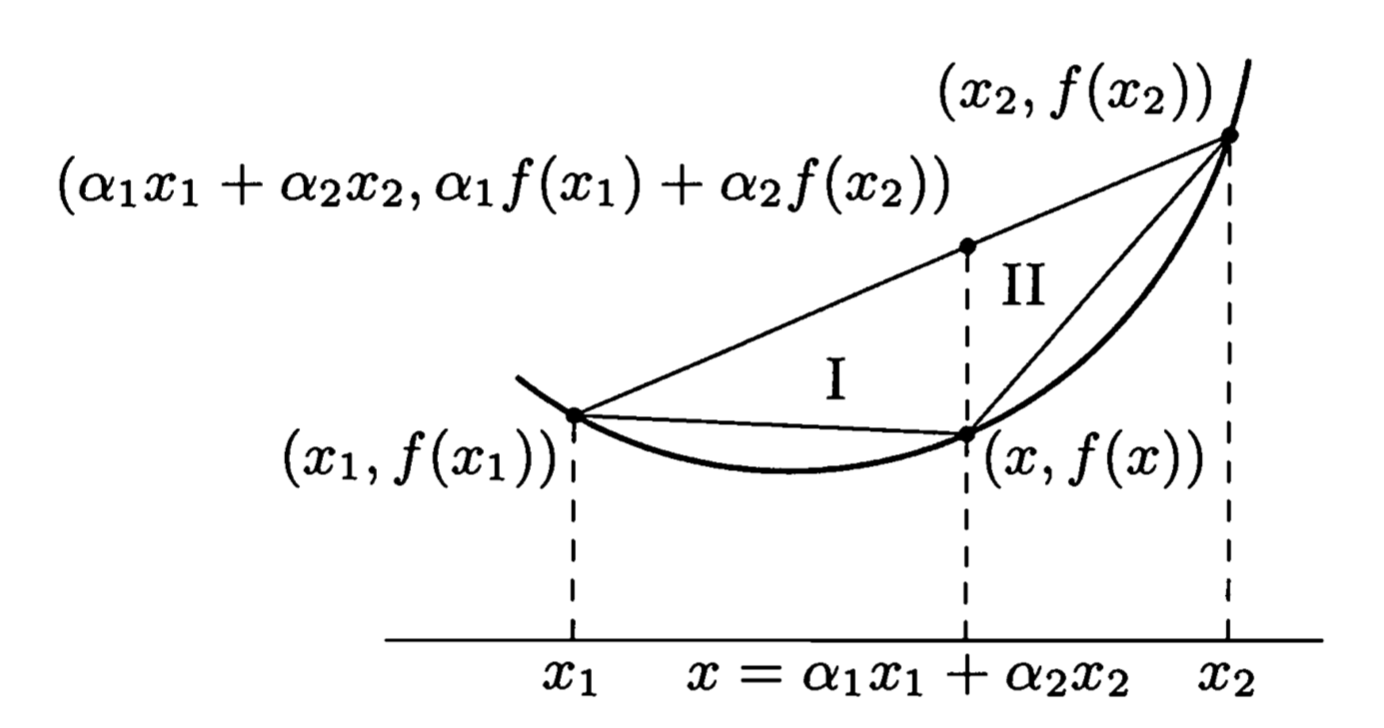
\includegraphics[width=0.5\textwidth]{convex.png}
    \caption{Convex function}
    \label{fig:fig2}
\end{figure}

\begin{definition}
    \normalfont 
    If the opposite inequality holds for a function $f: ]a,b[ \to \mathbb{R}$,
    that function is said to be concave on the interval $]a,b[$, or, more often,
    convex upward in the interval, as opposed to a convex function, which is 
    then said to be convex downward on $]a,b[.$
\end{definition}

In the relations $x = \alpha_1 x_1 + \alpha_2 x_2, \alpha_1 + \alpha_2 = 1,$ we have 
\[
    \alpha_1 = \frac{x_2 - x}{x_2 - x_1}, \alpha_2 = \frac{x - x_1}{x_2 - x_1}
    \]
so that formula~\ref{eq:eq8} can be rewritten as 
\[
    f(x) \le \frac{x_2 - x}{x_2 - x_1}f(x_1) + \frac{x - x_1}{x_2 - x_1}f(x_2)
    \]
Taking account the inequalities $x_1 < x < x_2$ and $x_1 < x_2$, we then 
obtain 
\[
    \left(x_2 - x\right)f(x_1) + \left(x_1 - x_2\right)f(x) + \left(x - x_1\right)f(x_2) \ge 0
    \]
Remarking that $x_2 - x_1 = (x_2 - x) + (x - x_1)$ we obtain from the last 
inequality, after elementary transformations 
\begin{equation}
    \frac{f(x) - f(x_1)}{x - x_1} \le \frac{f(x_2) - f(x_1)}{x_2 - x_1}
    \label{eq:eq9}
\end{equation}
for $x_1 < x < x_2$.

Inequality~\ref{eq:eq9} is another way of writing the definition of 
convexity of the function $f(x)$ on an open interval $]a,b[$. Geometrically,
\ref{eq:eq9} means (see Figure~\ref{fig:fig2})that the slope of the chord $I$
joining $x_1, f(x_1)$ to $x, f(x)$ is not larger than (and in the case of strict
convexity is less than) the slope of the chord $II$ joining $x, f(x)$ to $x_2, f(x_2)$.

Now let us assume that the function $f: ]a,b[ \to \mathbb{R}$ is differentiable 
on $]a,b[$. Then, letting $x$ in Eq.~\ref{eq:eq9} tend first to $x_1$, the tend 
to $x_2$, we obtain 
\[
    f'(x_1) \le \frac{f(x_2) - f(x_1)}{x_2 - x_1} \le f(x_2)
    \]
which establishes that the derivative of $f$ is monotonic.

Taking this fact into account, for a strictly convex function we find, using 
Lagrange's theorem, that 
\[
    f'(x_1) \le f'(\xi_1) = \frac{f(x) - f(x_1)}{x - x_1} < \frac{x_2 - x}{x_2 - x} = f'(\xi_2)
    \le f'(x_2)
    \]
for $x_1 < \xi_1 < x < \xi_2 < x_2$, that is, strict convexity implies that the derivative 
is strictly monotonic.

Thus, if a differentiable function $f$ is convex on an open interval $]a,b[$,
then $f'$ is nondecreasing on $]a,b[$, and in the case when $f$ is strictly convex, 
its derivative $f'$ is increasing on $]a,b[$.

These conditions turns out to be not only necessary, but also sufficient 
for convexity of a differentiable function.

\begin{proposition}
    \normalfont
    A necessary and sufficient condition for a function $f: ]a,b[ \to \mathbb{R}$
    that is differentiable on the open interval $]a,b[$ to be convex (downward)
    on that interval is that its derivative $f'$ be non-decreasing on $]a,b[$. 
    A strictly increasing $f'$ corresponds to a strictly convex function.
\end{proposition}

\begin{corollary}
    \normalfont
    A necessary and sufficient condition for a function $f: ]a,b[ \to \mathbb{R}$
    that having a second derivative on the open interval $]a,b[$ to be convex 
    on $]a,b[$ is that $f''(x) \ge 0$ on that interval. The condition $f''(x) > 0$
    on $]a, b[$ is sufficient to guarantee that $f$ is strictly convex.
\end{corollary}

\begin{example}
    \normalfont
    Let us examine the convex of the following functions:
    \[
     x^{\alpha}, a^x, \log_ax, \sin x
     \]
\end{example}

\begin{proposition}
    \normalfont
    A function $f: ]a,b[ \to \mathbb{R} $ that is differentiable on the open 
    interval $]a,b[$ is convex(downward) on $]a,b[$ if and only if its graph
    contains no points below any tangent drawn to it. In that case, a 
    necessary and sufficient condition for strict convexity is that all
    points of the graph except the point of tangency lie strictly above 
    the tangent line.
\end{proposition}

\begin{example}
    \normalfont
    Using the proposition to prove that 
    \[
        e^x \ge 1 + x 
        \]
    and this inequality is strict for $x \ne 0.$
    Similarly, using the convexity of $\ln x$, one can verify that 
    \[
        \ln x \le x - 1
        \]
    holds for $x > 0$, the inequality being strict for $x \ne 1$.
\end{example}

\begin{definition}
    \normalfont 
    Let $f: U(x_0) \to \mathbb{R}$ be a function defined and differentiable 
    on a neighborhood $U(x_0)$ of $x_0 \in \mathbb{R}$. If the function is 
    convex downward (resp. upward) on the set $\mathring{U}^-(x_0) =  
    \left\{x \in U(x_0) \vert x < x_0\right\}$ and convex upward (resp. downward)
    on $\mathring{U}^+(x_0) = \left\{x\in U(x_0) \vert x > x_0\right\} $, then $\left(x_0, f(x_0)\right)$
    is called an \textbf{infection point}.
\end{definition}

An analytic criterion for the abscissa $x_0$ of a point of infection 
is easy to surmise. If $f(x)$ is twice differentiable at $x_0$, then 
since $f'(x)$ has either a maximum or minimum at $x_0$, we must have $f''(x_0) = 0$.

If the second derivative $f''(x)$ is defined on $U(x_0)$ and one has 
one sign everywhere on $\mathring{U}^-(x_0)$ and the opposite sign on 
$\mathring{U}^+(x_0)$,so that the point $\left(x_0,f(x_0)\right)$ is a point of inflection.

\begin{example}
    When consider the function $f(x) = \sin x$, we shall show that 
    the abscissas $x = \pi k, k \in \mathbb{Z}$ are points of inflection.
\end{example}

\begin{example}
    \normalfont
    It should not be thought that the passing of a curve from one side 
    of its tangent line to the other at a point is a sufficient condition 
    for the point to be a inflection point. It may, after all, happen 
    that the curve does not have any constant convexity on either a 
    left or a right neighborhood of the point. A example (see Fig.~\ref{fig:fig3}) is 
    \[
        f(x) = \left\{\begin{array}{cl} 2x^3 + x^2\sin \frac{1}{x^2} & \text{ for } 
            x \ne 0, \\ 0 & \text{ for } x = 0 
        \end{array} \right.
        \]
    \label{ex:ex2}
\end{example}

\begin{proposition}{\rm \textbf{Jensen's Inequality}}
    \normalfont
    If $f: ]a,b[ \to \mathbb{R}$ is a convex function, $x_1, x_2, \cdots, x_n$ are points 
    of $]a,b[$, and $\alpha_1, \alpha_2, \cdots, \alpha_n$ are nonnegative numbers such that 
    $\alpha_1 + \alpha_2 + \cdots + \alpha_n = 1$, then 
    \[
        f(\alpha_1x_1 + \alpha_2x_2 + \cdots + \alpha_nx_n) \le \alpha_1f(x_1) + \alpha_2f(x_2) + \cdots + \alpha_nf(x_n)
        \]
\end{proposition}
\graphicspath{
    {./fun2/}
}
\begin{figure}[htbp]
    \centering
    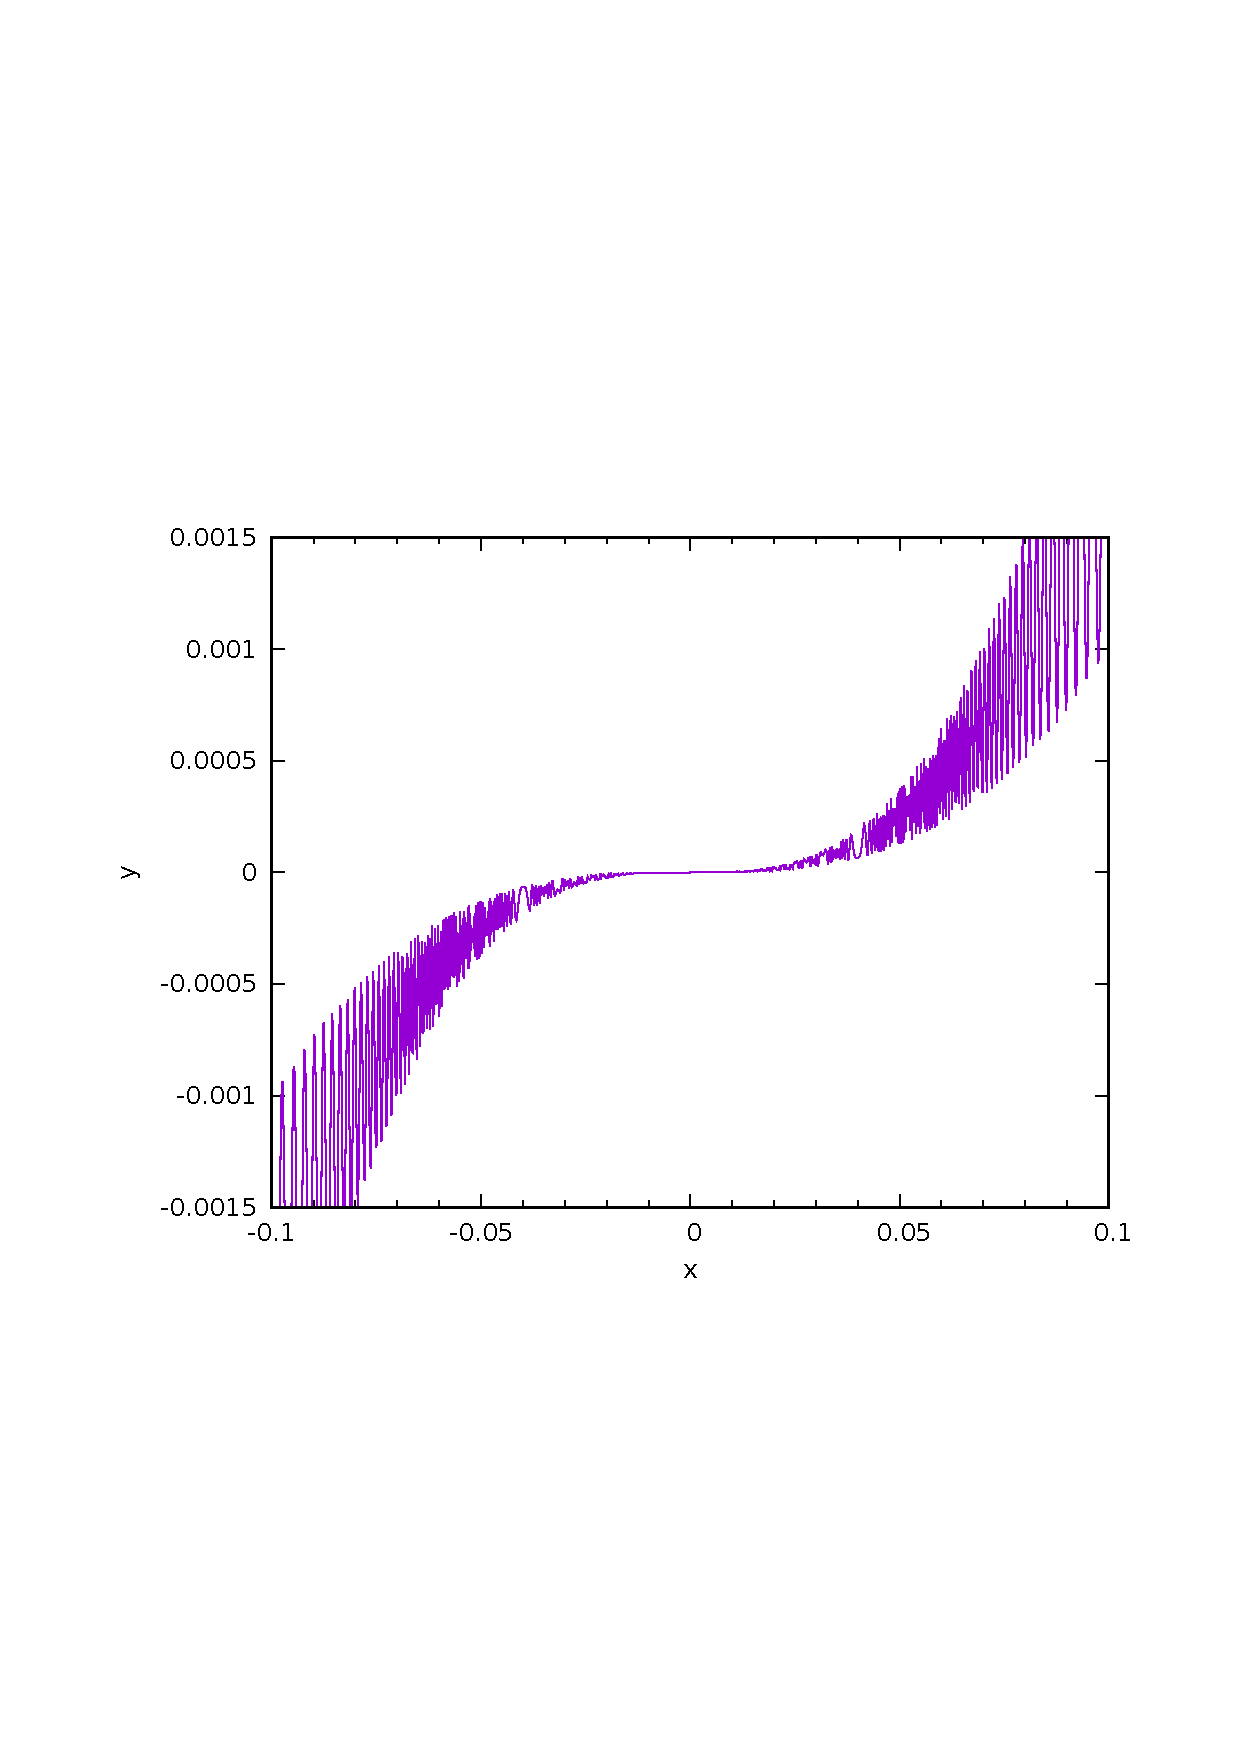
\includegraphics[height=0.4\textwidth]{fun2.pdf}
    \caption{Figure of example~\ref{ex:ex2}}
    \label{fig:fig3}
\end{figure}

\begin{example}
    \normalfont
    The function $f(x) = \ln x$ is strictly convex upward on the set of 
    positive numbers. ans so we have 
    \[
        \alpha_1\ln x_1 + \alpha_2\ln x_2 + \cdots + \alpha_n\ln x_n \le \ln\left(\alpha_1x_1 + \alpha_2x_2 
        + \cdots + \alpha_nx_n\right)
        \]
    or 
    \[
        x_1^{\alpha_1} x_2^{\alpha_2} \cdots x_n^{\alpha_n} \le \alpha_1x_1 + \alpha_2x_2 + \alpha_nx_n
        \]
    for $x_i \ge 0, i=1,2,\cdots,n, \sum_{i=1}^n\alpha_i = 1$.
    In partiular, if $\alpha_i = \frac{1}{n}, i=1,2,\cdots,n$, we obtain the classical 
    inequality 
    \[
        \sqrt[n]{x_1x_2\cdots x_n} \le \frac{x_1 + x_2 + \cdots + x_n}{n}
        \]
\end{example}

\begin{example}
    \normalfont
    Let $f(x) = x^p, x \ge 0, p>1$. Since such a funtion is convex, we have 
    \[
        \left(\sum_{i=1}^n\alpha_i x_i\right)^p \le \sum_{i=1^n}\alpha_ix_i^p.
        \]
    Setting $\displaystyle q = \frac{p}{p-1}, \alpha_i = b_i^q\left(\sum_{i=1}^nb_i^q\right)^{-1}$, and 
    $\displaystyle x_i = a_ib_i^{-1/(p_i-1)}\sum_{i=1}^nb_i^q$ here, we obtain the Holder's 
    inequality:
    \[
        \sum_{i=1}^na_ib_i \le \left(\sum_{i=1}^na_i^p\right)^{1/p}\left(\sum_{i=1}^na_i^q\right)^{1/q}
        \]
\end{example}

\section{L'H$\ddot{\rm \textbf{o}}$spital Role}
We now pause to discuss a special, but very useful device for finding 
the limit of a ratio of functions, known as L'Hospital 
\footnote{G.F.de l'Hospital(1661-1704), French mathematician, a capable 
student of Johann Bernoulli.}rule.

\begin{proposition}
    \normalfont 
    Suppose the functions $f: ]a,b[ \to \mathbb{R}$ and $g: ]a,b[ \to \mathbb{R}$
    are differentiable on the open interval $]a,b[$ with $g'(x) \ne 0$ on $]a,b[$
    and 
    \[
        \frac{f'(x)}{g'(x)} \to A \text{ as } x \to a+0 (-\infty \le A \le +\infty),
        \]
    then 
    \[
        \frac{f(x)}{g(x)} \to A \text{ as } x \to a+0
        \]
    in each of the following two cases:
    \begin{enumerate}
        \item $\displaystyle f(x) \to 0 \wedge g(x) \to 0, \text{ as } x \to a+0,i$
        \item $\displaystyle g(x) \to \infty, \text{ as } x \to a+0.$
    \end{enumerate}
    A similar assertion holds as $x \to b-0$.
\end{proposition}
\begin{proof}
    \normalfont
    \[
        \frac{f(x) - f(y)}{g(x) - g(y)} = \frac{f'(\xi)}{g'(\xi)}
        \]
    \[
        \frac{f(x)}{g(x)} = \frac{f(y)}{g(x)} + \frac{f'(\xi)}{g'(\xi)}
        \left(1 - \frac{g(y)}{g(x)}\right)
        \]
\end{proof}

\begin{example}
    \normalfont 
    Find the following limits using L'Hospital rule.
    \[
        \lim_{x \to 0}\frac{1 - \cos 2x}{x^2}
        \]
    \[
        \lim_{x \to \infty}\frac{\frac{\pi}{2} - \tan^{-1}x}{\sin \frac{1}{x}}
        \]
    \[
        \lim_{x \to +\infty}\frac{x^a}{e^{bx}},(a>0,b>0)
        \]
    \[
        \lim_{x \to 0}x \ln x
        \]
    \[
        \lim_{x \to 0^+}\ln^x\frac{1}{x}
        \]
    \[
        \lim_{x \to 0}x^x
        \]
    \[
        \lim_{x\to {\frac{\pi}{2}}}\frac{1 + \sin x}{1 - \cos x}
        \]
    \[
        \lim_{x \to \infty} \frac{x + \cos x}{x}
        \]
\end{example}
\section{Asymptotic Line}
\begin{definition}
    \normalfont 
    The line $c_0 + c_1x$ is called the \textbf{asympotote} of the graph of 
    the function $y = f(x)$ as $x \to -\infty$(or $x \to +\infty$) if 
    \[
        f(x) - (c_0 + c_1x) = \circ(1) \text{ as } x \to -\infty (or x \to +\infty)
        \]
    \label{def:def1}
\end{definition}
It obviously from the Def.\ref{def:def1} that 
\[
    c_1 = \lim_{x \to -\infty}\frac{f(x)}{x}
    \]
and 
\[
    c_0 = \lim_{x \to -\infty} \left(f(x) - c_1x\right)
    \]
In general, if $\displaystyle f(x) - (c_0 + c_1x + \cdots + c_nx^n) = 0$
as $x \to -\infty$, then 
\[
    c_n = \lim_{x \to -\infty}\frac{f(x)}{x^n}
    \]
\[
    c_{n-1} = \lim_{x \to -\infty} \frac{f(x) - c_nx^n}{x^{n-1}}
    \]
\[
    \vdots\]
\[
    c_0 = \lim_{x \to -\infty} f(x) - (c_1x + c_2x^2 + \cdots + c_nx^n)
    \]
These relations, written out here for $x \to -\infty$, are of course also 
valid in the case $x \to +\infty$ and can be used to describe the asymptotic 
behavior of the graph of a function $f(x)$ using the graph of the 
corresponding algebraic polynomial $c_0 + c_1x + \cdots + c_nx^n$.

\begin{example}
    \normalfont
    The graph of the function 
    \[
        y = x + \tan^{-1}(x^3 - 1)
        \]
    is well approximated by the line $y = x - \frac{\pi}{2}$,
    as $x \to -\infty$, and by the line $y = x + \frac{\pi}{2}$, as 
    $x \to +\infty$.
\end{example}

\subsection{Examples of Sketches of Graphs of Functions(
Without Application of the Differential Calculus)}
\begin{example}
    \normalfont
    Let us construct a sketch of the graphs of the functions 
    \[
        h = \log_{x^2-3x -2}2
        \]
    \[
        y = \sin x^2
        \]
\end{example}

\graphicspath{ 
    {./Figs/}
}
\begin{figure}
    \centering
    \begin{minipage}[htbp]{0.4\textwidth}
        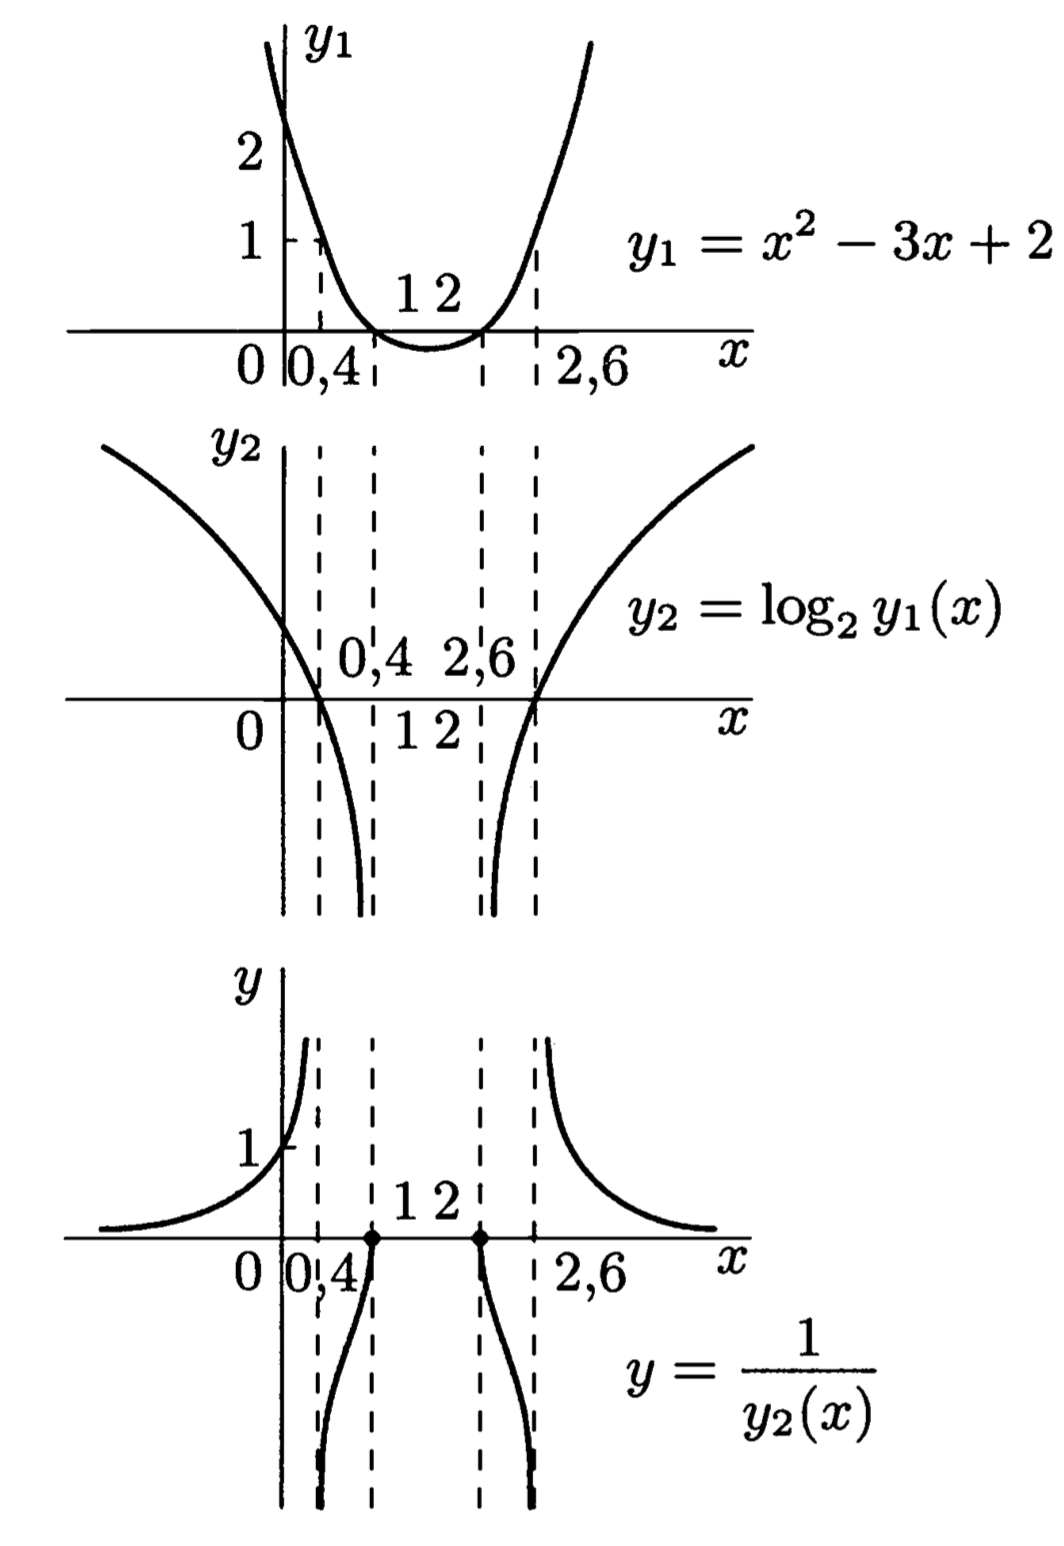
\includegraphics[width = \textwidth]{funplot1.png}
        \caption{Graph of $\log_{x^2 - 3x -2}2$}
    \end{minipage}
    \begin{minipage}[htbp]{0.4\textwidth}
        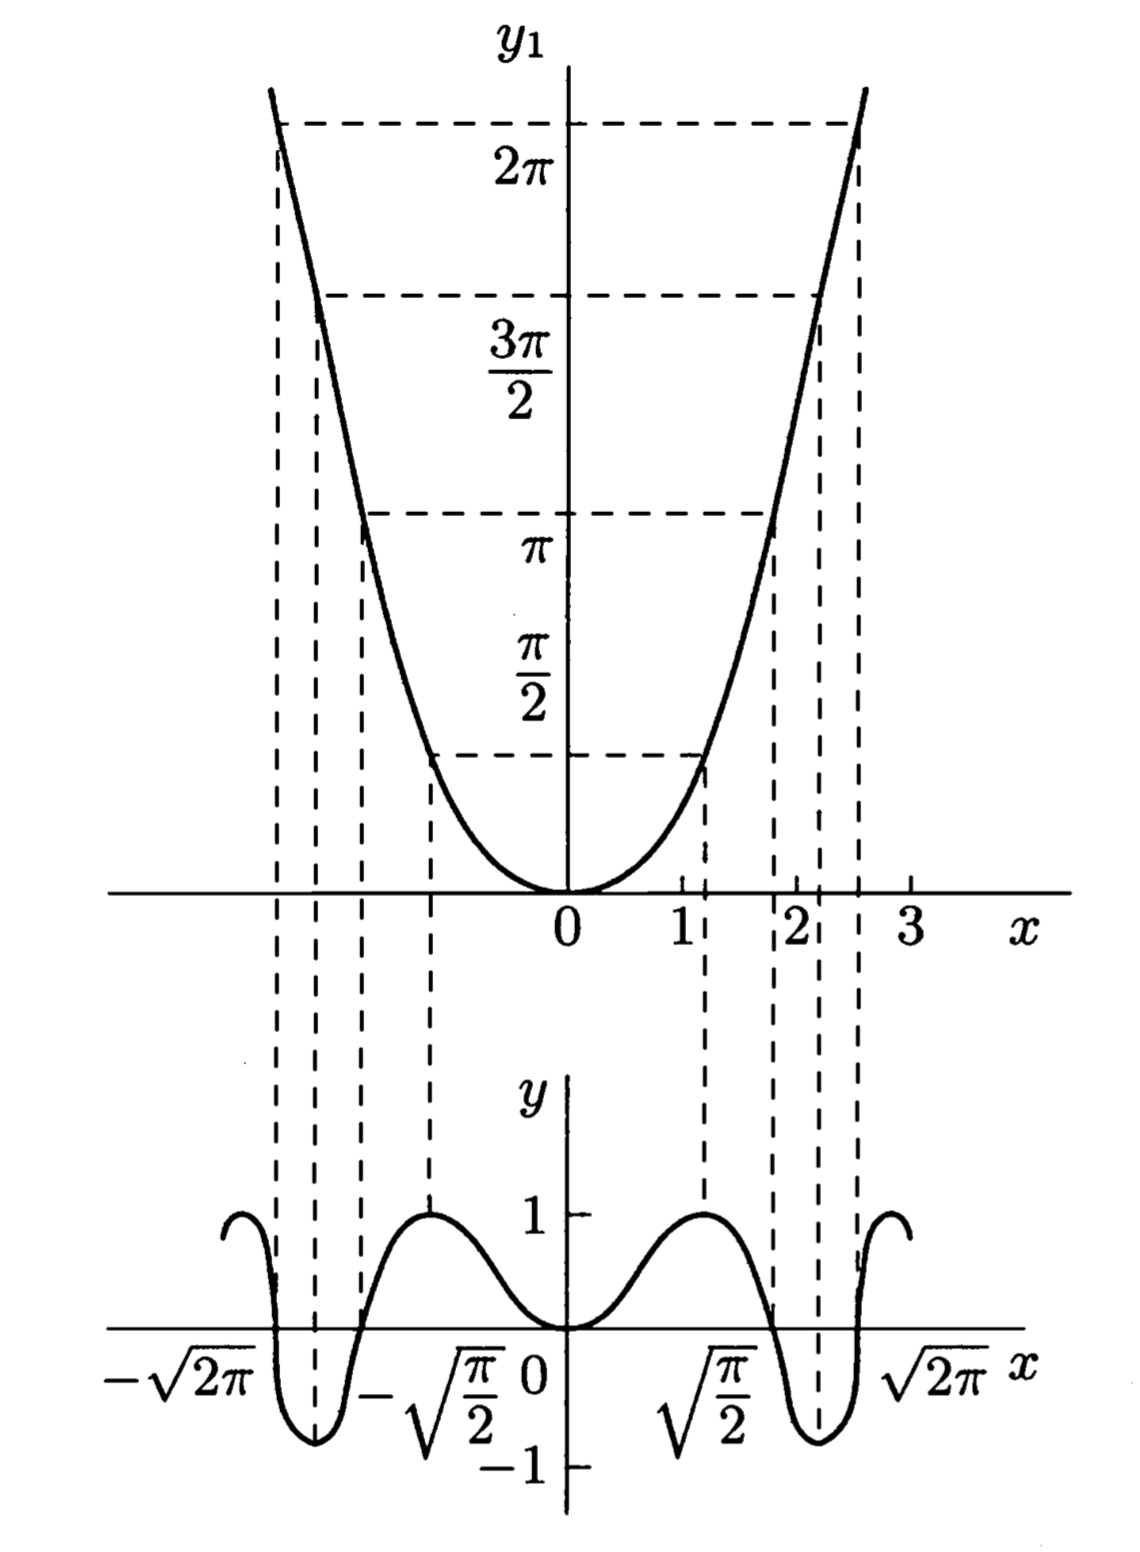
\includegraphics[width = \textwidth]{funplot2.png}
        \caption{Graph of $\sin x^2$}
    \end{minipage}
    \label{fig:fig4}
\end{figure}

\subsection{The Use of Differential Calculus in Constructing 
the Graph of a Function}
\begin{example}
    \normalfont
    Construct the graph of the function (see Figure~\ref{fig:fig5})
    \[
        f(x) = \vert x + 2 \vert e^{-1/x}
        \]
    \label{ex:ex3}
\end{example}
\begin{figure}[htbp]
    \centering
    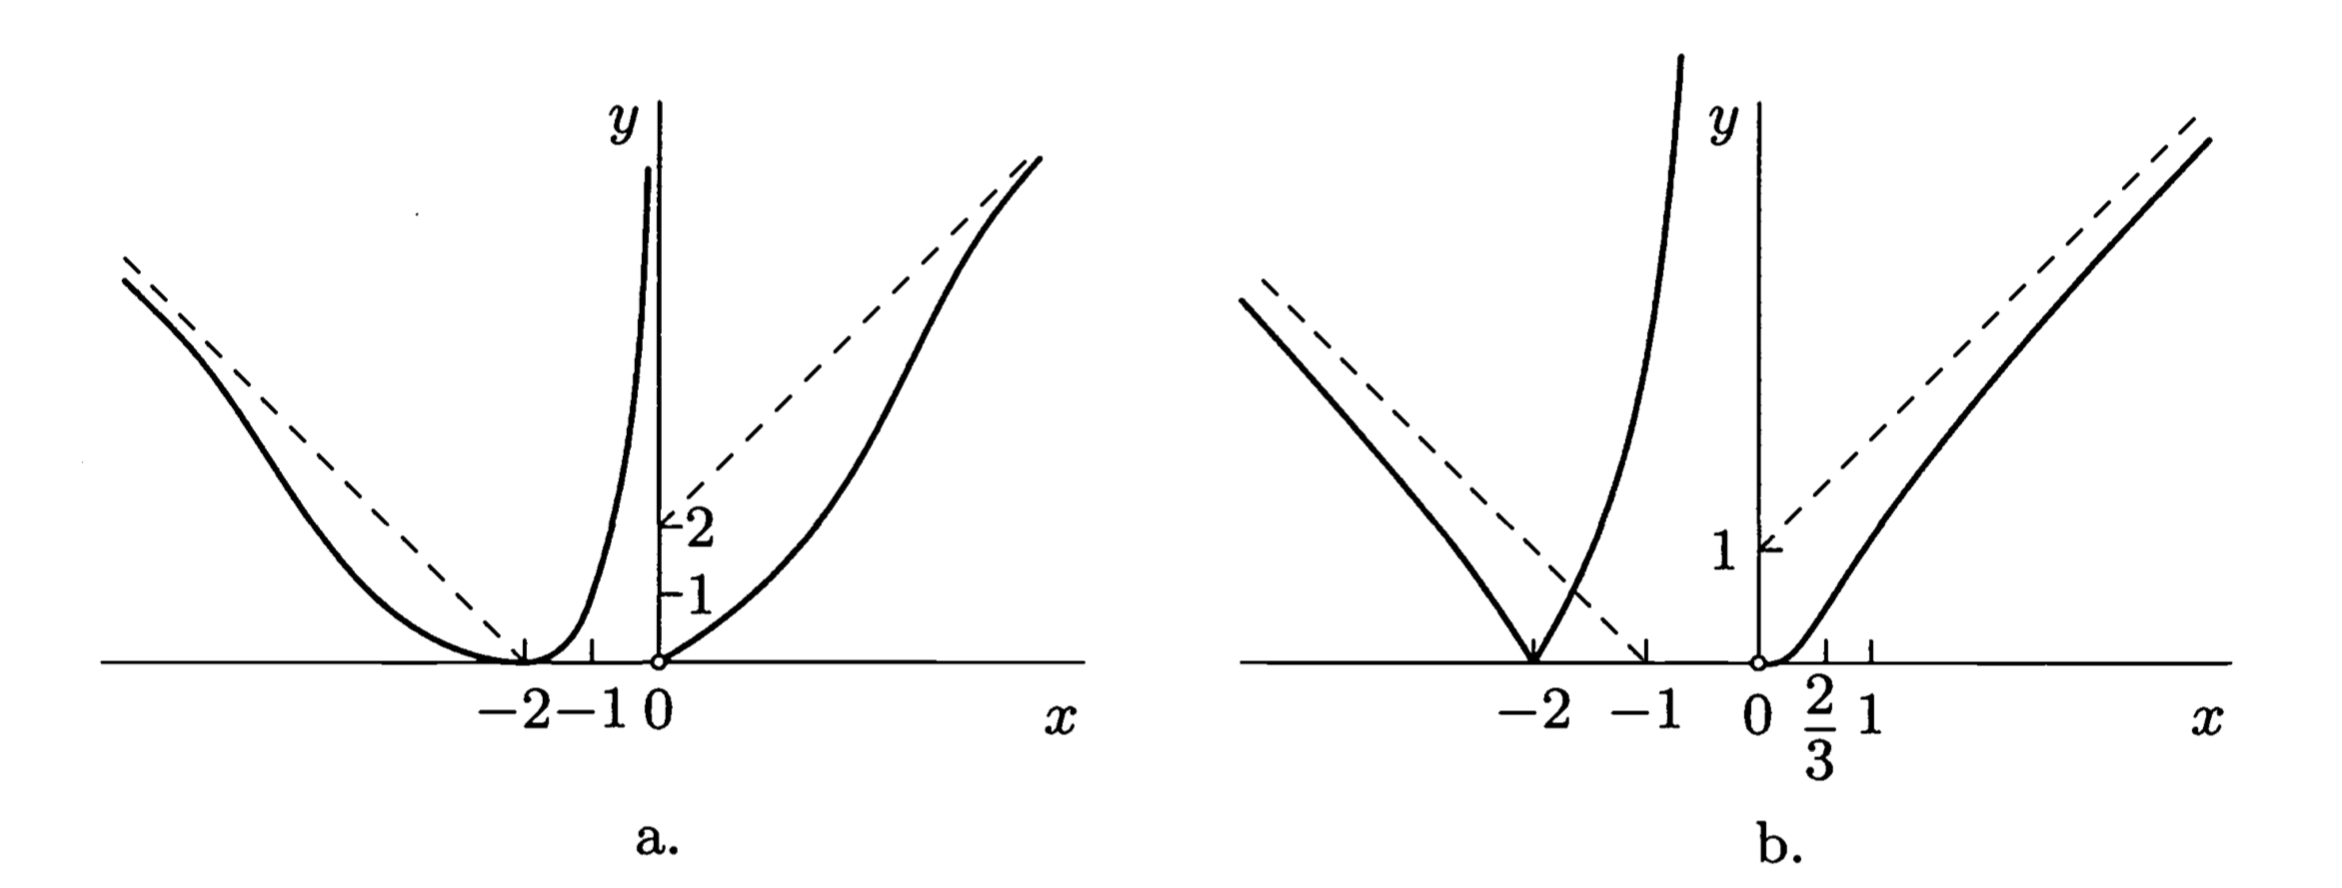
\includegraphics[width = \textwidth]{funplot3.png}
    \caption{Graph of the function example~\ref{ex:ex3}}
    \label{fig:fig5}
\end{figure}
    









\end{document}
